Como mencionamos, nos interesa saber que heuristica de búsqueda local se adapta mejor aplicada a alguna de las familias estudiadas con el algoritmo del ejercicio 2. Para esto, las enunciaremos nuevamente:

\begin{enumerate}
\item Elección de gimansios con cero poder 
\item Anillos de pokeparadas y gimansios
\item Entrada fuera de orden (orden diferente para lograr el óptimo)
\item Movida segura
\item Hay un quinto!!!
\item Y capaz un sexto!!!
\end{enumerate}

Las familias de casos que no tienen solución (y por lo tanto no se puede aplicar búsqueda local) o las que proveen la solución óptima, serán descartadas. En el caso de las soluciones óptimas, dado que ya sabemos que lo son y los algoritmos de busqueda local tienen un tiempo de corrida prefijado, por lo que no se puede observar nada interesante de estos casos.\\
Por lo tanto, nos centraremos en las familias enumeradas anteriormente para ver cual de las búsquedas locales puede obtener una solución mejor a la solución provista por el algoritmo $greedy$. O en caso de no poder mejorarla, trataremos de dar respuesta a los motivos.\\

Se tomarán 30 mediciones por búsqueda local. Se tomará una media alfa podada de las mismas con $\alpha$ = 0.5 de manera de podar un 25\% de los datos a cada lado. De esta forma se reducen los outliers en las muestras consideradas. 
Además se tomará la varianza muestral usando la media calculada y las mediciones que queden luego de aplicar la media.\\

\subsubsection*{Familia 1}

\vspace*{0.3cm} \vspace*{0.3cm}
  \begin{center}
 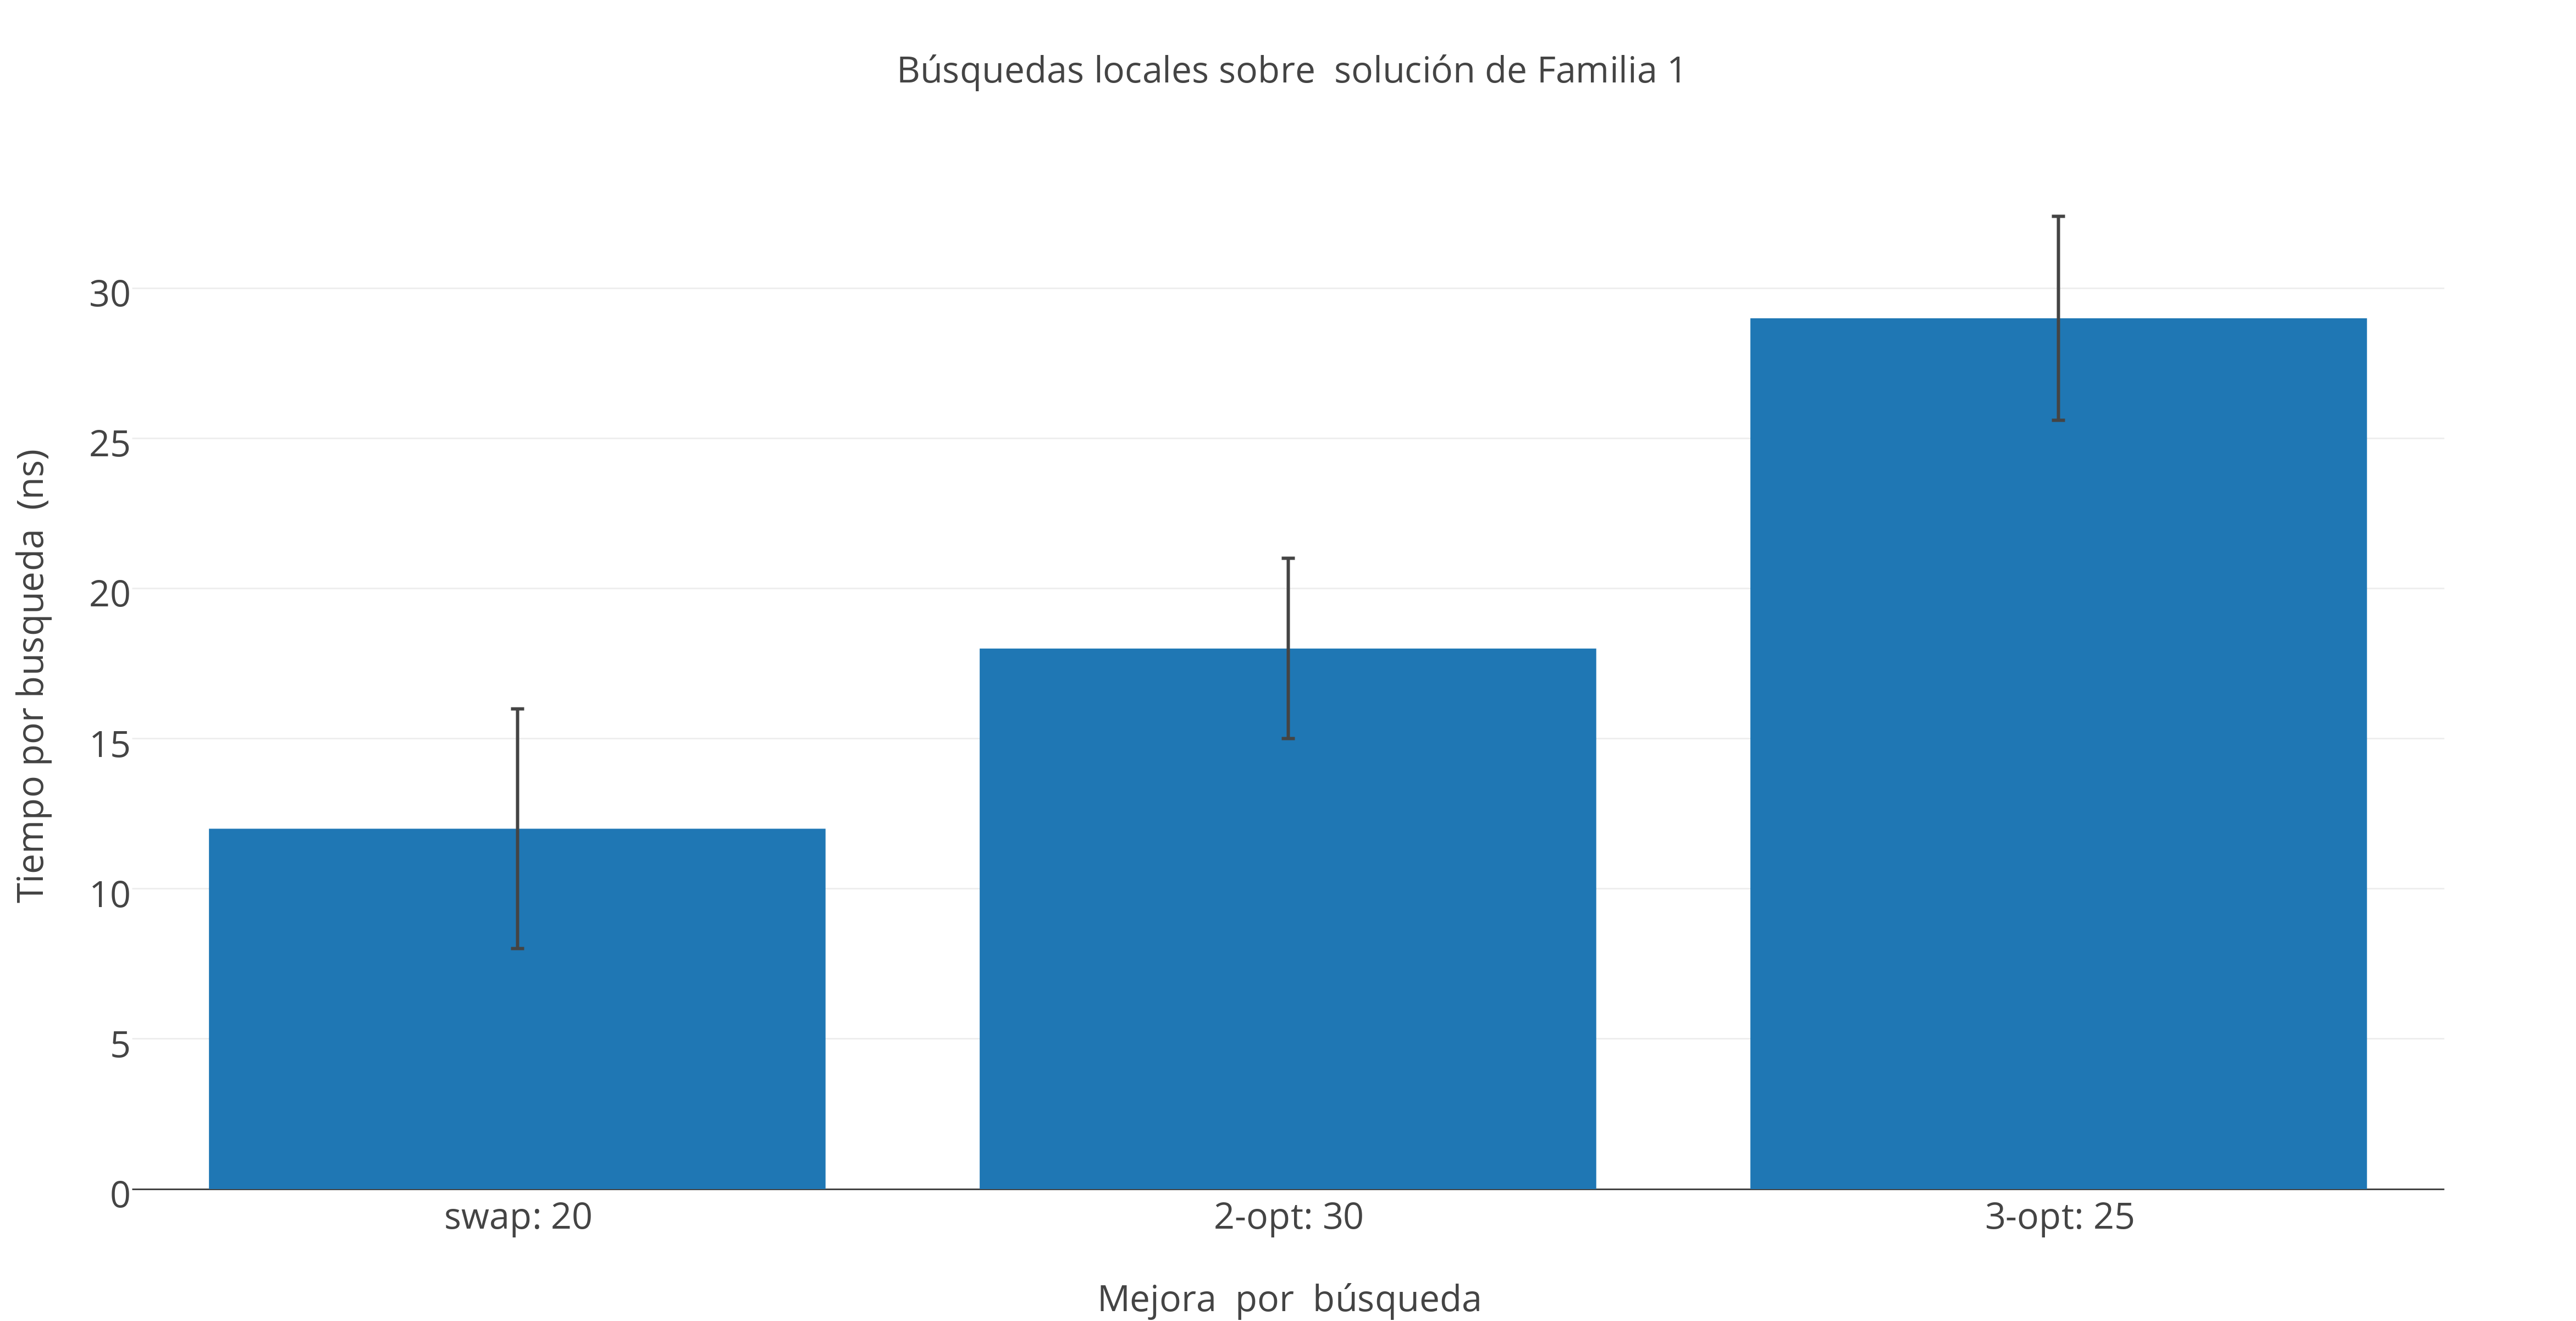
\includegraphics[scale=0.5]{./EJ3/local_search_familia.png}
 {            \textit{Gráfico \ 3.1 - Búsquedas locales sobre Familia 1}}
  \end{center}
  \vspace*{0.3cm}
  
SEGURAMENTE SON MAS CASOS O POR FAMILIA O MAS FAMILIAS! TESTEAR TODAS Y OBTENER CONCLUSIONES
